%! Author = partsjoo
%! Date = 16.04.2023

\newpage


\section{Scenario description}
Imagine the following situation. A number of farmers want to share their farming practices with each other, in order to improve yields. They want to figure out, when, what and how much to plant; when and how much to fertilize, when to harvest, etc. These predictions (i.e. a model is going to be built, using machine learning) are based on their previous practices (what operations they performed, and what was the resulting yield), considering that different fields may have been subject to different external conditions (previous years; crops, rainfall, insolation, etc.), and may also have different quality of soil. The farmers consider their previous actions and the resulting yields their private information. The descriptions of external conditions are not really secret, but their historic values may be most straightforwardly obtainable from companies that specialize in gathering and cleaning up such data (e.g. satellite pictures, weather conditions from various times in the past) and make the selling of resulting datasets their business; these companies should also be involved in building the farming models.
In the end, a farmer should be able to query that model with the parameters of the field (its location, and the characteristics of its soil), the expected weather for the upcoming growing season, and the crop they intend to grow on this field, and receive back suggestions on how to plant this crop and what activities to plan during the growing season. The data from other farmers, and the queries from other farmers should still remain private.


\begin{enumerate}
  \item Please suggest how the computation should be set up and which PETs should be used.
  \item How would you use these technologies, and how do you select the parameters?
  \item Which technologies would likely not give a significant boost to privacy?
  \item Consider the likely wishes of the users, as well as the legislative requirements.
  \item Discuss the possible channels through which privacy might be compromised.
  \item Try to estimate numeric parameters where appropriate (where the techniques use them or where the adversary can be characterized numerically).
  \item Propose a couple (e.g., three) alternative solutions and compare their pros and cons against each other.
  \item Draw conceptual diagrams (using stick figures, UML, (PE-)BPMN, or something else) of your proposed solutions, showing which data moves from which party to which other party.
\end{enumerate}


\section{Scenario analysis}

\subsection{Differential Privacy (DP)}
Differential privacy allows data to be analyzed and shared while preserving individual privacy.
It introduces noise into the data, limiting the disclosure of individual records.


\begin{figure}[!htbp]
  \centering
  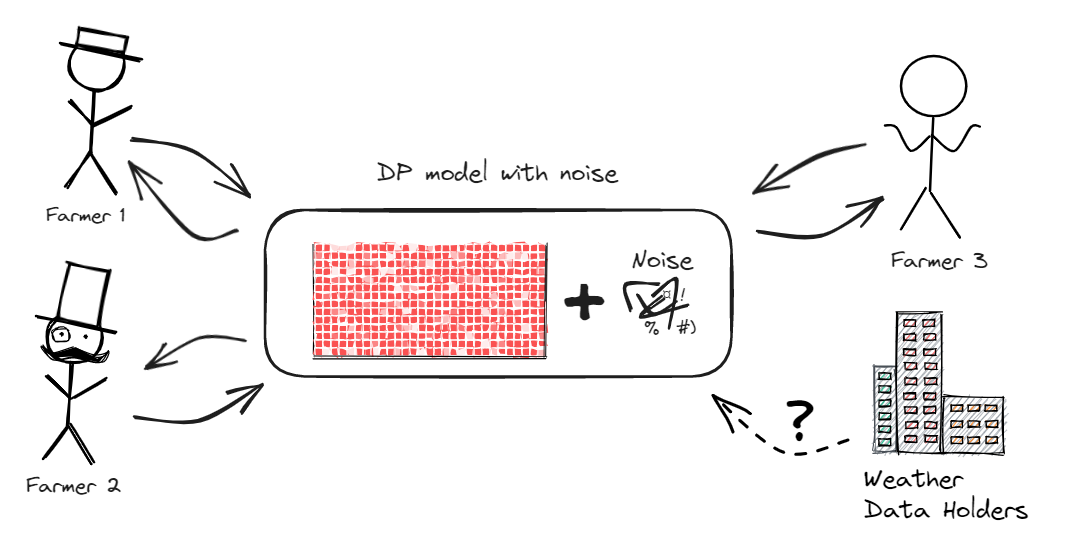
\includegraphics[width=\textwidth]{assets/img_3}
  \caption{Example of using DP with noise to produce a model.}
  \label{fig:img_3}
\end{figure}

Application: Here, differential privacy could be applied when creating models for farming practices.
A model could be built based on the combined, noisy data from all farmers.
When queried, this model could provide useful suggestions without revealing individual contributions.
Noise parameters should be chosen such that enough privacy is guaranteed
(a typical value for ε, the privacy budget, could be 1.0, but this depends on the precise requirements and available data volume).

Limitations: Too much noise can reduce the utility of the data.
Models can be very sensitive to noise, especially for small datasets.
And also the noise added to the data afterward can also be sensitive (e.g. imagine the model answering to use fertilizer amount X but the
X can be 1 or 0).
The trade-off between privacy and utility must be carefully managed.
It might not be sufficient for strong legal requirements.

\subsection{Fedearated Learning (FL)}
Federated learning is a machine learning approach where a model is trained across multiple decentralized devices
(or servers) holding local data samples, without exchanging them.

\begin{figure}[!htbp]
  \centering
  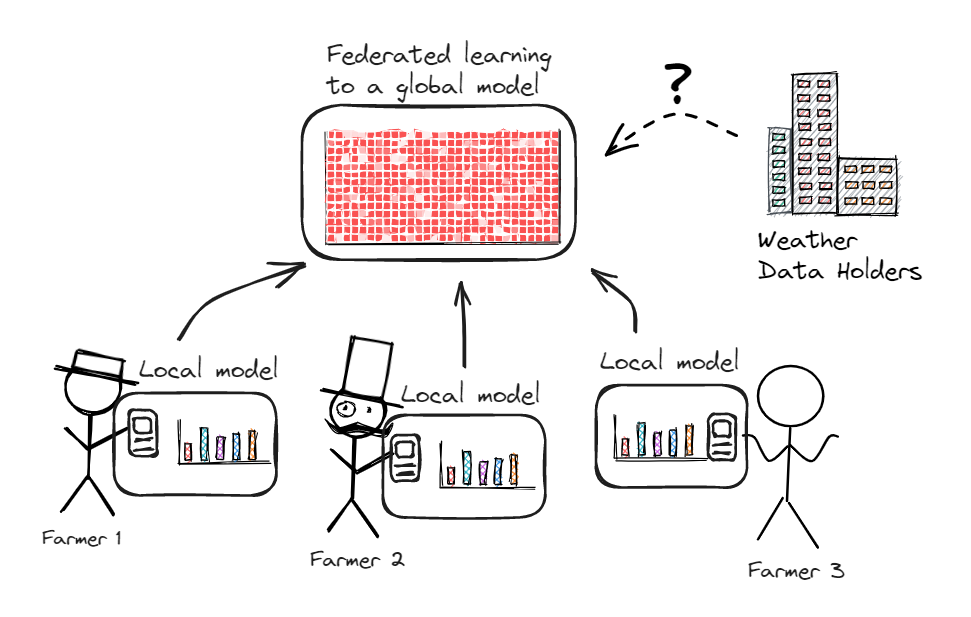
\includegraphics[width=\textwidth]{assets/img_2}
  \caption{Example of using Federated Learning to produce a global model.}
  \label{fig:img_2}
\end{figure}

Application: Each farmer could train a local model based on their own data, and only the model parameters would
be shared and aggregated to form a global model.
In this case, farmers' data never leaves their premises.

Limitations: It requires that each participant has the resources to train a local model,
which might not be feasible for every farmer.
Also, complex models may still leak some private information. Another issue here is how to choose the model workflow?
Should it be syncronized - can models be trained in an aggregation server or can it be even peer-to-peer. Google has showed that
this could be one viable way by training models on local mobile devices~\cite[]{mcmahan2017communication}.

\subsection{Multi-Party Computation (MPC)}
MPC allows multiple parties to compute a function over their inputs while keeping those inputs private.

\begin{figure}[!htbp]
  \centering
  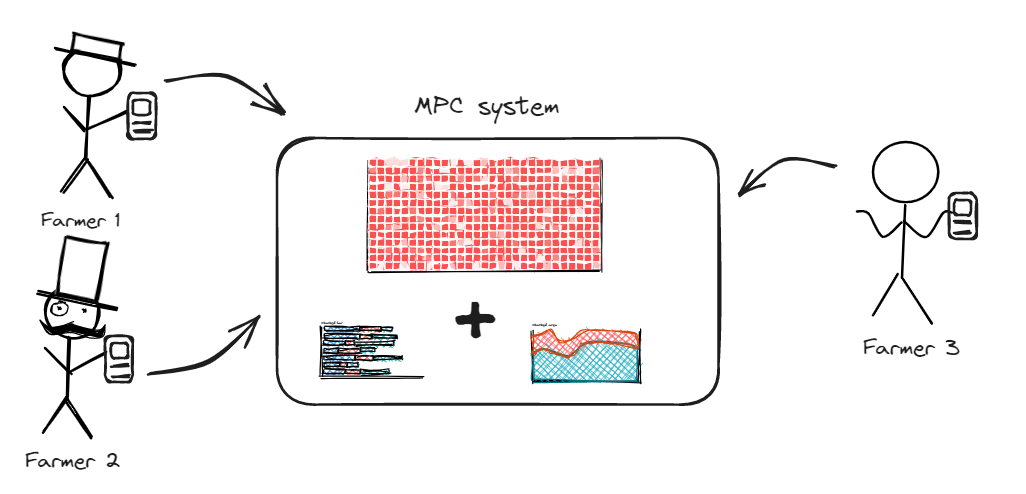
\includegraphics[width=\textwidth]{assets/img_4}
  \caption{Example of using MPC.}
  \label{fig:img_4}
\end{figure}

Application: MPC can be used to compute the desired farming models in a way that no participant learns anything about the others'
inputs (aside from what can be inferred from the result).
The data from the farmers and the weather data providers can be used as inputs.

Limitations: MPC can be computationally expensive and slow, especially for complex machine learning models.
It also requires trust in the system's setup (honest majority of participants, secure communication channels, etc.) so if were talking about
a large number of farmers (an assuming the average farmer wouldn't have high trust towards anyone), this might not be feasible.

Potential privacy leaks could occur through side channels or through inference from the results
(e.g., if one farmer has very unique data). Also, the choice of parameters (like the noise in differential privacy, or the security parameters in MPC)
can impact the privacy-utility trade-off.

\subsection{Other things to consider}

\textbf{Data amount to transfer should be minimal because farmers don't have computing power.} Let's consider the situation with 100 farmers
who
want to share their farming practices. Each farmer has collected data on 10,000 individual crop plants, resulting in a dataset of 1,000,000 records. Each record contains 10 fields, including the type of crop, the amount of fertilizer used, the amount of water used, the temperature, the amount of sunlight, the soil pH, and the yield. The data is highly sensitive as it includes specific farming techniques and the yield, which could give competitors an edge.
Transfering large armounts of data can also be expensive, so it might be better to transfer only the model parameters. If we go that
route we
could use \textbf{homomorphic encryption} to compute the model parameters without decrypting the data. This significantly reduces the
amount of
data sent over the network, but it can be computationally expensive. It also saves the farmers from having a powerful machine to train
the model, which kind of makes it hard to set up a FL system. Homomorphic encryption can be a good choice for small sets in certain
scenarios because it
provides a way to perform computations on
encrypted data without the need for decryption, thus preserving privacy.~\cite[]{10.1007/978-3-642-37682-5_1}
Though for this to work we would probably have to standarize some kind of form to be filled by the farmers, so that the
amount of data to encrypt is small and \textbf{uniform}.

For all methods the risk to data privacy with small datasets is twofold the way I see it.

First(limited data), the limited volume of data might increase the likelihood
of identifying individual data points or making inferences about individuals, particularly if the dataset includes unique or rare
characteristics (regional specific drought, or other extremely specific regional macro events). If there are two major competitors in
the country and one of them has a very specific data point, it might be possible to infer that this data point belongs to that competitor.

Second(exposed data points), in the context of machine learning, smaller datasets could lead to overfitting,
where the model learns specific details and noise, potentially exposing individual data patterns and thereby compromising privacy.

Lastly, if one of the farmers is malicious, they could try to infer information about other farmers' data by providing the model with
'known' data about the competitor, and then observing the model's output. This is called a membership inference attack.

Questions I asked myself but don't have answers to: How to validate trained model when the output can't be compared to the training set,
because training
set
is
unreadble? One way could be
with 'k' subsets or folds of the data perhaps? The model is trained on 'k-1' folds and then validated on the remaining fold.

\section{Main solution: secure aggregation}

\begin{figure}[!htbp]
  \centering
  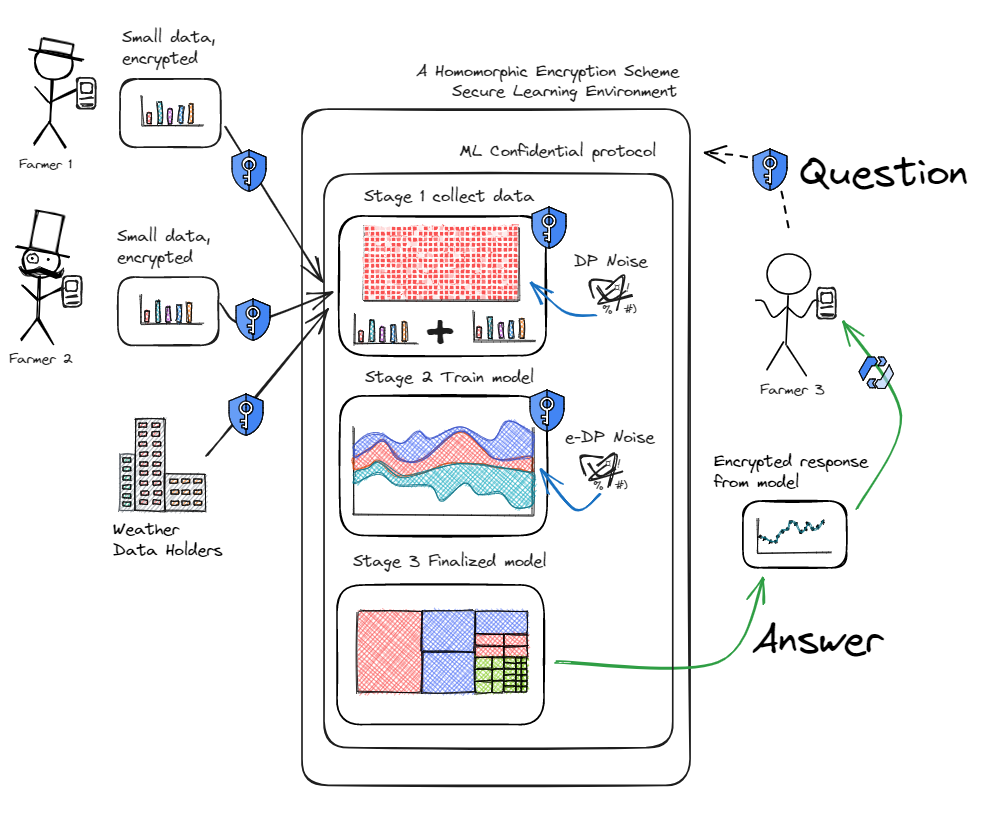
\includegraphics[width=\textwidth]{assets/img_7}
  \caption{Using homomorpich encryption to train ML model in a secure environment with encrypted data only.}
  \label{fig:img_7}
\end{figure}

Initially, farmers, acting as data owners, gather uniform and relatively small-sized data points from their day-to-day farming practices. These may include variables such as crop type, planting dates, amount of fertilizer used, and crop yield, among others. These raw data are then encrypted utilizing a homomorphic encryption scheme. Homomorphic encryption allows computations to be performed directly on the encrypted data, thus ensuring the privacy of the original information throughout the transmission and processing stages.

For the transfer of the data some secure protocol should be used HTTPS, VPN etc.

This is also good from a legal perspective because the data is encrypted and the farmer is the only one who has the key to decrypt it.
Data used is minimized. Only the necessary data required for training the model is collected. Though with little context to the data (
size is small and uniformed) the usefulness of the model might be limited.

The encrypted data are securely transmitted to a cloud-based server referred to as the 'Secure Learning Environment', which is managed by
a trusted Cloud Service Provider. This server is designed to safeguard the confidentiality of the farmers' data throughout the machine
learning process. In theory, it should be possible to securely aggregate
data while ensuring that clients’ inputs are only learned by the
server in aggregate.~\cite[]{bonawitz2017practical}

In parallel with the transmission of the farmers' data, external companies specializing in the gathering and cleaning of environmental data, act as content providers. They supply additional homomorphically encrypted data to the Secure Learning Environment. These data points, encompassing variables such as historical and current weather conditions, insolation, and other external environmental parameters, are integrated with the farmers' data.

Within the Secure Learning Environment, these combined data are used to train a machine learning model. The model can be then queried
from a centralized location, and the results can be sent back to the farmers.

The privacy training model will use Privacy-Preserving Machine Learning (PPML)~\cite[]{SESTAK2021459}. By adding DP-based noise to the
training data to not so complex data otherwise should give a good trade-off between privacy and utility.

For example: farmers, acting as data owners, gather an average of $n = 1000$ small-sized data points daily from their farming practices. These may include variables such as crop type, planting dates, amount of fertilizer used ($F_{avg} = 50,kg$ per acre), and crop yield ($Y_{avg} = 2000,kg$ per acre), among others.

In the Secure Learning Environment, data from $m = 100$ farmers, and additional homomorphically encrypted data from environmental data providers are used to train a machine learning model. Considering the combined data from all sources, the total data used for training amounts to $(n \times m) + E_{data} = 100,000 + 10,000 = 110,000$ data points, where $E_{data}$ represents the environmental data points.

The introduction of DP noise to the dataset is performed to ensure the privacy of the individual farmer's data. Let's denote $\epsilon$ as the DP privacy parameter. With a higher $\epsilon$, less noise is added, resulting in better model utility but lower privacy. Conversely, a lower $\epsilon$ leads to more noise, enhancing privacy at the cost of model utility.

To illustrate this, let's consider three scenarios with $\epsilon_1 > \epsilon_2 > \epsilon_3$. For $\epsilon_1$, the noise introduced may be minimal, leading to a more accurate model (with negligible loss, let's say $L_{\epsilon_1} = 0.05$) but weaker privacy guarantees. On the other hand, $\epsilon_2$ might lead to a moderate amount of noise addition, balancing between data utility and privacy, with a slightly higher model loss $L_{\epsilon_2} = 0.15$. Lastly, $\epsilon_3$ would introduce a large amount of noise, ensuring strong privacy but with an increased model loss ($L_{\epsilon_3} = 0.30$) due to the effect of noise on model training.

The concern that the environmental data points could be used to infer the other farmers' data is legitimate. However, by incorporating DP, we add an additional layer of privacy protection. The noise added to the dataset effectively 'blurs' the unique characteristics of individual farmer data, making it challenging for an adversary to infer specific farmer data even if they have access to the environmental data.

It is also important to note that some utility loss is an expected outcome in the modeling process.
The goal is to find a balanced trade-off point where the privacy assurance is satisfactory without overly sacrificing the model's predictive performance.

\newpage
\section{Alternative solution: Fedearated Learning with MPC}

We use Region 1 and Region 2, for a more secure and decentralized training of the machine learning model, leveraging the data from farmers'
practices. This structure ensures the confidentiality of farmers' data as it remains within their respective region and is not directly
exposed to the global network. I constraint adding the localized (regional) data to the global model only if the MPC has determined that
the model data is big enough to be added to the global model. This prevents the previously mentioned membership inference attack.
Downside is ofcurse, clients might wait a long time for the model to be updated.

\begin{figure}[!htbp]
  \centering
  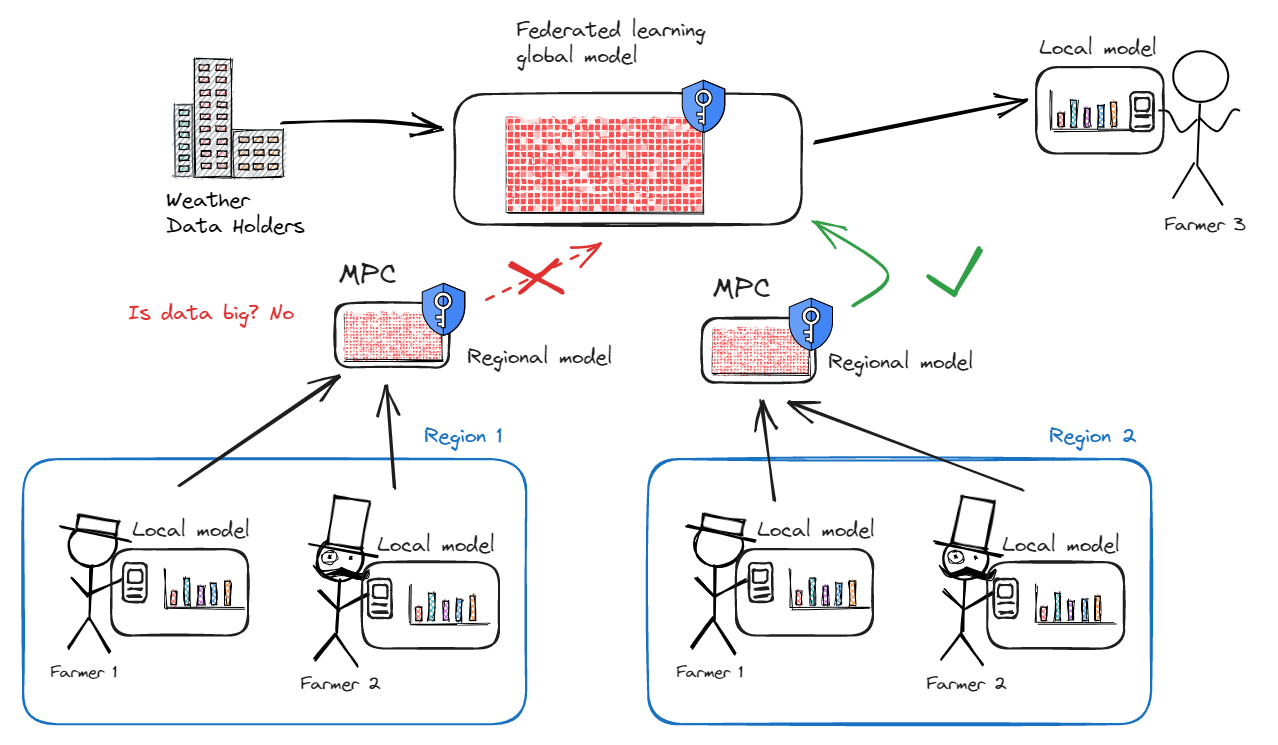
\includegraphics[width=\textwidth]{assets/img_9}
  \caption{Using MPC to train ML model locally and only adding it to the global model if set is beg enough.}
  \label{fig:img_9}
\end{figure}

Each regional model, trained on localized and specialized data, adds an extra layer of granularity to the
general model. These independently trained regional models are then aggregated into a federated learning network. This aggregation
process is designed to maintain the privacy of the underlying data, with each regional model contributing to the global model without exposing its raw data.

Secure Multi-Party Computation (SMPC) is utilized. In this scenario, both the data owner (for instance, a farmer requesting an inference
from the model) and the model owner aim to keep their information confidential: the farmer input data and the model, respectively.

This process begins with the data owner and the model owner encrypting their respective data/model using secret sharing.
The concept of secret sharing revolves around splitting the data/model into shares that do not contain any usable information on their own and thus can be safely exchanged with the other party.
Following this, inference is conducted by jointly computing a function (in this case, the neural network inference procedure) using SMPC.
The data owner then receives an encrypted result, which only they can decrypt, thereby maintaining the confidentiality of the data and the model throughout the process.

By the time localized model becomes availiable in the global model, the data is already encrypted and the model is already trained. This
could be futher improved by adding some noise to the data before training the model, though I don't it's explicitly necessary, because
aggregating several models should already provide some noise to the data by itself.

Problem with this apporach is that the if someone from Region 1 makes a query they might get highly inaccurate results, because their
location specific data is not present in the global model. Other issue is also that computing power is shifted more towards the farmers(
though they don't compute, they just send the data to the MPC, but still they need to have a powerful enough machine to encrypt and
transfer large amounts of data).

The good thing is that that can also be done even if the farmers willingness to share data is low, because instead of sharing the data,
they are sharing the trained ML model.~\cite[]{mo2022sok}

\section{Alternative solution: Training the model in an trusted execution environment}
Though the last example is much of a stretch, I think it's worth mentioning.
The idea is to train the model in a trusted execution enviorment specifically designed to protect the data and the model.
Users add their data into the TEE and the model is trained there.
Additonally, the input data is first stripped of sensitive information and then synthetic data is produced from it
while maintaining statistical properties of the original data.

\begin{figure}[!htbp]
  \centering
  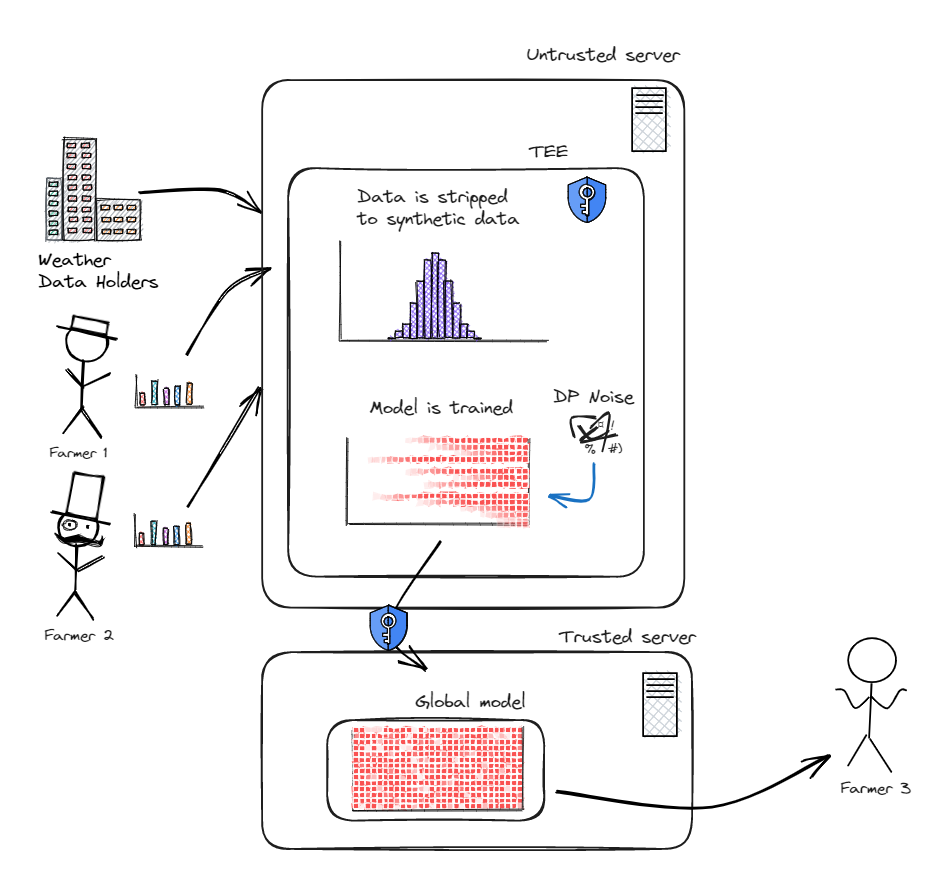
\includegraphics[width=\textwidth]{assets/img_10}
  \caption{Using MPC to train ML model locally and only adding it to the global model if set is beg enough.}
  \label{fig:img_10}
\end{figure}

In this final scenario, we envisage a situation where farmers provide their data to an untrusted server equipped with a Trusted Execution Environment (TEE).
TEEs allow for the execution of code in an isolated and secure enclave, with the results being confidential from the hardware provider.

Farmers' data is transmitted to the server and then converted into synthetic data within the TEE, thus maintaining the privacy of the original data.
Synthetic data maintains the statistical characteristics of the original data without directly exposing any sensitive information, thereby providing an additional layer of privacy.
Within the TEE, a machine learning model is trained using this synthetic data.
Post-training, the model is made available on the trusted server as a global model, ready for use while ensuring data privacy.

The concept of differential privacy (DP) also plays a vital role in this process. DP provides a formal guarantee that models trained on similar datasets are indistinguishable.
DP is realized by adding noise to the synthetic data, which can blur the specifics. Running a DP training
algorithm in a TEE ensures that the DP mechanism is faithfully applied, thereby adding another level of privacy assurance.

The upside of this is that the computation speed for the model will be good, because the model is trained on a powerful machine. The
downside of course is that farmers have to trust the TEE provider, which is not always the case.
However TEEs are vulnerable to various side- and covert-channel attacks, physical attacks, confused deputy attacks, Denial-of-Service (
DoS) attacks, etc.~\cite[]{mo2022sok}

Overall, the combination of TEE and DP, along with the use of synthetic data, can create a secure and private environment for machine learning applications.
This way, farmers can comfortably share their data with the assurance that their data privacy is maintained and contribute to the global model.
